\documentclass[10pt,english,twocolumn,fleqn]{extarticle}

\usepackage{geometry}
\geometry{verbose,tmargin=1.0cm,bmargin=1.5cm,lmargin=0.8cm,rmargin=0.8cm}
\setlength{\parskip}{\smallskipamount}
\setlength{\parindent}{0pt}

\usepackage{tikz}

\begin{document}

\begin{figure}
\centering
\input{line_1}
\par
\caption{Lines}
\end{figure}

\begin{figure}
\centering
\input{line_2}
\par
\caption{Arrows}
\end{figure}

\begin{figure}
\centering
\begin{tikzpicture}
\draw [<->] (1,2) -- (0,0) -- (3,0);
\end{tikzpicture}

\par
\caption{Arrows 2nd}
\end{figure}

\begin{figure}
\centering
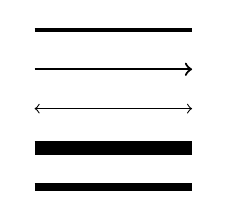
\begin{tikzpicture}
\draw [ultra thick] (0,1) -- (2,1);
\draw [thick,->] (0,0.5) -- (2,0.5);
\draw [thin,<->] (0,0) -- (2,0);
\draw [line width=5] (0,-0.5) -- (2,-0.5);
\draw [line width=0.1cm] (0,-1) -- (2,-1);
\end{tikzpicture}

\par
\caption{Test thickness}
\end{figure}

\begin{figure}
\centering
\begin{tikzpicture}
\draw [dashed, ultra thick] (0,1) -- (2,1);
\draw [dashed,->] (0,0.5) -- (2,0.5);
\draw [dotted] (0,0) -- (2,0);
\end{tikzpicture}

\par
\caption{Dashes and dots}
\end{figure}

\begin{figure}
\centering
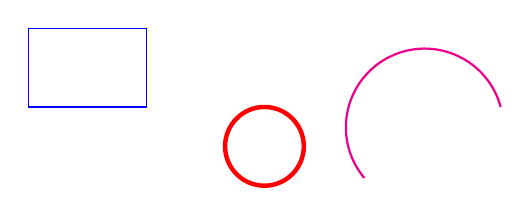
\begin{tikzpicture}
\draw [blue] (0,0) rectangle (1.5,1);
\draw [red,ultra thick] (3,-0.5) circle [radius=0.5];
\draw [magenta,thick] (6,0) arc [radius=1, start angle=15, end angle=220];
\end{tikzpicture}

\par
\caption{Curves 1}
\end{figure}

\begin{figure}
\centering
\input{curve_2}
\par
\caption{Curves 2}
\end{figure}

\begin{figure}
\centering
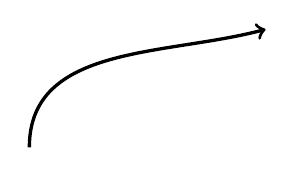
\begin{tikzpicture}
\draw [very thick,->] (0,0) to [out=90,in=195] (3,1.5);
\end{tikzpicture}

\par
\caption{Curves 3}
\end{figure}

\begin{figure}
\centering
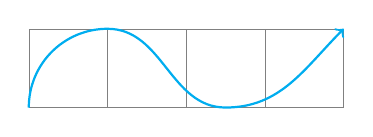
\begin{tikzpicture}
\draw [help lines] (0,0) grid (4,1);
\draw [->, thick, cyan] (0,0) to [out=90,in=180] (1,1)
      to [out=0,in=180] (2.5,0) to [out=0,in=-135] (4,1);
\end{tikzpicture}

\par
\caption{Curves 4}
\end{figure}

\begin{figure}
\centering
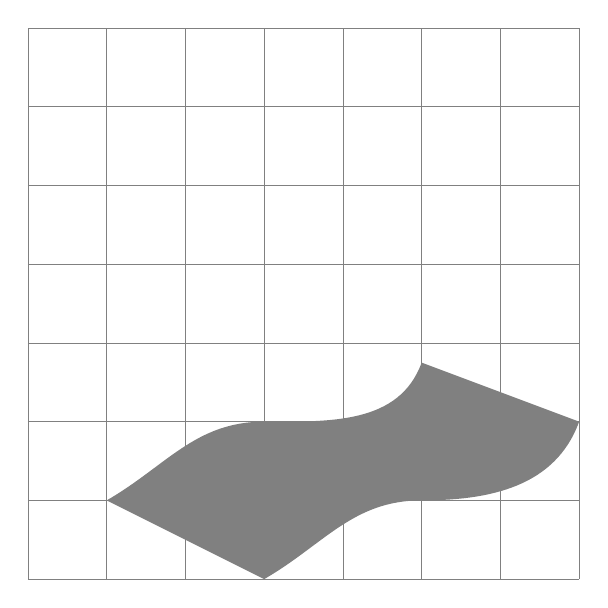
\begin{tikzpicture}
\draw [help lines] (-1,-1) grid (6,6);
\path [fill=gray,thick] (0,0) -- (2,-1) to [out=30,in=180] (4,0)
      to [out=0,in=250] (6,1) -- (4,1.75)
      to [out=250,in=0] (2,1) to [out=180,in=30] (0,0);
\end{tikzpicture}

\par
\caption{Curve 5}
\end{figure}

\begin{figure}
\centering
\input{func_1}
\par
\caption{Function 1}
\end{figure}

\begin{figure}
\centering
\input{func_2}
\par
\caption{Function 2}
\end{figure}


\begin{figure}
\centering
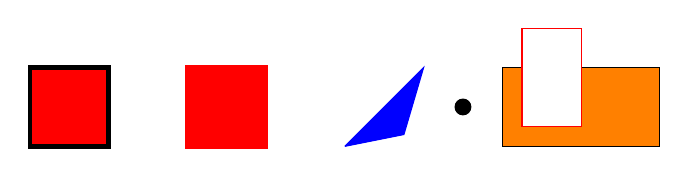
\begin{tikzpicture}
\draw [fill=red, ultra thick] (0,0) rectangle (1,1);
\draw [red, fill=red, ultra thick] (2,0) rectangle (3,1);
\draw [blue, fill=blue] (4,0) -- (5,1) -- (4.75,0.15) -- (4,0);
\draw [fill] (5.5,0.5) circle [radius=0.1];
\draw [fill=orange] (6,0) rectangle (8,1);
\draw [red, fill=white] (6.25,0.25) rectangle (7,1.5);
 \end{tikzpicture}

\par
\caption{Fill 1}
\end{figure}

\begin{figure}
\centering
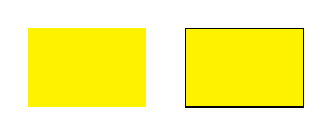
\begin{tikzpicture}
\path [fill=yellow] (0,0) rectangle (1.5,1);
\draw [fill=yellow] (2,0) rectangle (3.5,1);
\end{tikzpicture}

\par
\caption{Fill 2}
\end{figure}

\begin{figure}
\centering
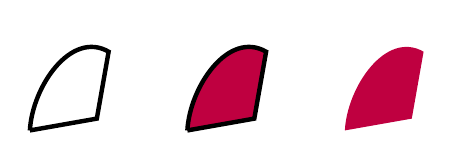
\begin{tikzpicture}
\draw [ultra thick] (0,0) to [out=87,in=150] (1,1) -- (0.85,0.15) -- (0,0);
\draw [ultra thick, fill=purple] (2,0) to [out=87,in=150] (3,1) -- (2.85,0.15) -- (2,0);
\path [fill=purple] (4,0) to [out=87,in=150] (5,1) -- (4.85,0.15) -- (4,0);
\end{tikzpicture}

\par
\caption{Fill 3}
\end{figure}

\begin{figure}
\centering
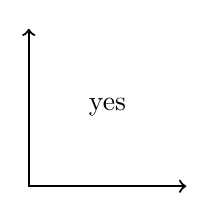
\begin{tikzpicture}
\draw [thick,<->] (0,2) -- (0,0) -- (2,0);
\node at (1,1) {yes};
\end{tikzpicture}

\par
\caption{Label 1}
\end{figure}

\begin{figure}
\centering
\input{label_2}
\par
\caption{Label 2}
\end{figure}

\begin{figure}
\centering
\input{label_3}
\par
\caption{Label 3}
\end{figure}

\begin{figure}
\centering
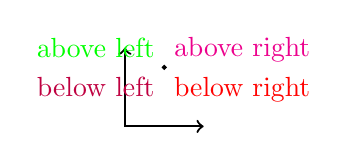
\begin{tikzpicture}
\draw [thick,<->] (0,1) -- (0,0) -- (1,0);
\draw [fill] (0.5,0.75) circle [radius=0.025];
\node [below right, red] at (0.5,0.75) {below right};
\node [above left, green] at (0.5,0.75) {above left};
\node [below left, purple] at (0.5,0.75) {below left};
\node [above right, magenta] at (0.5,0.70) {above right};
\end{tikzpicture}

\par
\caption{Label 4}
\end{figure}

\begin{figure}
\centering
\begin{tikzpicture}
\draw [thick,<->] (0,3) -- (0,0) -- (3,0);
\node [below right] at (3,0) {$x$};
\node [left] at (0,3) {$y$};
\draw [fill] (1.4,1.6) circle [radius=0.5pt];
\node [above right] at (1.4,1.6) {$A$};
\end{tikzpicture}

\par
\caption{Label 5}
\end{figure}

\begin{figure}
\centering
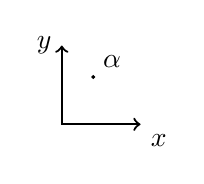
\begin{tikzpicture}
\draw [thick,<->] (0,1) node [left] {$y$} -- (0,0) -- (1,0) node [below right] {$x$};
\draw [fill] (0.4,0.6) circle [radius=0.5pt] node [above right] (0.4,0.6) {$\alpha$};
\end{tikzpicture}

\par
\caption{Label 6}
\end{figure}

\begin{figure}
\centering
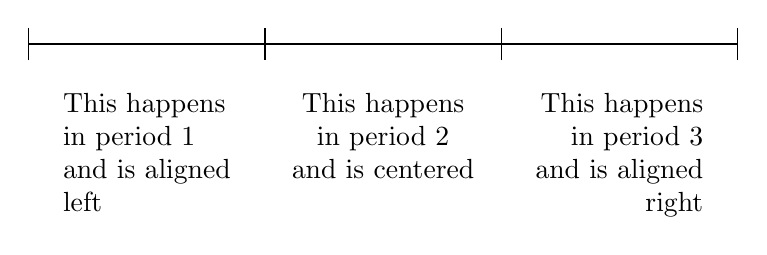
\begin{tikzpicture}
\draw [thick] (0,0) -- (9,0);
\draw (0,-0.2) -- (0,0.2);
\draw (3,-0.2) -- (3,0.2);
\draw (6,-0.2) -- (6,0.2);
\draw (9,-0.2) -- (9,0.2);
\node[align=left, below] at (1.5,-0.5) {This happens\\in period 1\\and is aligned\\left};
\node[align=center, below] at (4.5,-0.5) {This happens\\in period 2\\and is centered};
\node[align=right, below] at (7.5,-0.5) {This happens\\in period 3\\and is aligned\\right};
\end{tikzpicture}

\par
\caption{Label 7}
\end{figure}

\end{document}
